\documentclass[a4paper,11pt]{scrartcl}
\usepackage[a4paper, left=2cm, right=4.5cm, top=2cm, bottom=2cm]{geometry} % kleinere Ränder

%Paket für Header in Koma-Klassen (scrartcl, scrrprt, scrbook, scrlttr2)
\usepackage[headsepline]{scrlayer-scrpage}
% Header groß genug für 3 Zeilen machen
\setlength{\headheight}{3\baselineskip}


% Default Header löschen
\pagestyle{scrheadings}
\clearpairofpagestyles

% nicht kursiv gedruckte header
\setkomafont{pagehead}{\sffamily\upshape}

% Links im Dokuement sowie \url schön machen
\usepackage[colorlinks,pdfpagelabels,pdfstartview = FitH, bookmarksopen = true,bookmarksnumbered = true, linkcolor = black, plainpages = false, hypertexnames = false, citecolor = black]{hyperref}

% Umlaute in der Datei erlauben, auf deutsch umstellen
\usepackage[utf8]{inputenc}
\usepackage[ngerman]{babel}

% Mathesymbole und Ähnliches
\usepackage{amsmath}
\usepackage{mathtools}
\usepackage{amssymb}
\usepackage{microtype}
\newcommand{\NN}{{\mathbb N}}
\newcommand{\RR}{{\mathbb R}}
\newcommand{\QQ}{{\mathbb Q}}
\newcommand{\ZZ}{{\mathbb{Z}}}

% Komplexitätsklassen
\newcommand{\pc}{\ensuremath{{\sf P}}}
\newcommand{\np}{\ensuremath{{\sf NP}}}
\newcommand{\npc}{\ensuremath{{\sf NPC}}}
\newcommand{\pspace}{\ensuremath{{\sf PSPACE}}}
\newcommand{\exptime}{\ensuremath{{\sf EXPTIME}}}
\newcommand{\CClassNP}{\textup{NP}\xspace}
\newcommand{\CClassP}{\textup{P}\xspace}

% Weitere pakete
\usepackage{multicol}
\usepackage{booktabs}

% Abbildungen
\usepackage{tikz}
\usetikzlibrary{arrows,calc}





% Meistens ist \varphi schöner als \phi, genauso bei \theta
\renewcommand{\phi}{\varphi}
\renewcommand{\theta}{\vartheta}

% Aufzählungen anpassen (alternativ: \arabic, \alph)
\renewcommand{\labelenumi}{(\roman{enumi})}

% rwth colors
% colors: blue violet purple carmine red magenta orange yellow grass cyan gold silver
\definecolor{rwth-blue}{cmyk}{1,.5,0,0}\colorlet{rwth-lblue}{rwth-blue!50}\colorlet{rwth-llblue}{rwth-blue!25}
\definecolor{rwth-violet}{cmyk}{.6,.6,0,0}\colorlet{rwth-lviolet}{rwth-violet!50}\colorlet{rwth-llviolet}{rwth-violet!25}
\definecolor{rwth-purple}{cmyk}{.7,1,.35,.15}\colorlet{rwth-lpurple}{rwth-purple!50}\colorlet{rwth-llpurple}{rwth-purple!25}
\definecolor{rwth-carmine}{cmyk}{.25,1,.7,.2}\colorlet{rwth-lcarmine}{rwth-carmine!50}\colorlet{rwth-llcarmine}{rwth-carmine!25}
\definecolor{rwth-red}{cmyk}{.15,1,1,0}\colorlet{rwth-lred}{rwth-red!50}\colorlet{rwth-llred}{rwth-red!25}
\definecolor{rwth-magenta}{cmyk}{0,1,.25,0}\colorlet{rwth-lmagenta}{rwth-magenta!50}\colorlet{rwth-llmagenta}{rwth-magenta!25}
\definecolor{rwth-orange}{cmyk}{0,.4,1,0}\colorlet{rwth-lorange}{rwth-orange!50}\colorlet{rwth-llorange}{rwth-orange!25}
\definecolor{rwth-yellow}{cmyk}{0,0,1,0}\colorlet{rwth-lyellow}{rwth-yellow!50}\colorlet{rwth-llyellow}{rwth-yellow!25}
\definecolor{rwth-grass}{cmyk}{.35,0,1,0}\colorlet{rwth-lgrass}{rwth-grass!50}\colorlet{rwth-llgrass}{rwth-grass!25}
\definecolor{rwth-green}{cmyk}{.7,0,1,0}\colorlet{rwth-lgreen}{rwth-green!50}\colorlet{rwth-llgreen}{rwth-green!25}
\definecolor{rwth-cyan}{cmyk}{1,0,.4,0}\colorlet{rwth-lcyan}{rwth-cyan!50}\colorlet{rwth-llcyan}{rwth-cyan!25}
\definecolor{rwth-teal}{cmyk}{1,.3,.5,.3}\colorlet{rwth-lteal}{rwth-teal!50}\colorlet{rwth-llteal}{rwth-teal!25}
\definecolor{rwth-gold}{cmyk}{.35,.46,.7,.35}
\definecolor{rwth-silver}{cmyk}{.39,.31,.32,.14}

% 请把新添加的宏包放置此处
%\usepackage{blindtext} 
\usepackage{enumitem}
%\usepackage {ctex} % 中文字体支持
\usepackage[most]{tcolorbox} 
% https://tex.stackexchange.com/questions/180325/boxed-equation-with-number/180326
% http://mirrors.dotsrc.org/ctan/macros/latex/contrib/mathtools/empheq.pdf#page=23

\tcbset{colback=rwth-blue!10!white, colframe=-rwth-red!50!black, 
	highlight math style= {enhanced, %<-- needed for the ’remember’ options
		colframe=red,colback=red!10!white,boxsep=0pt}
} 
%   for tcolorbox
% 	Example
%	\begin{tcolorbox}[ams gather*]
%		\sum\limits_{n=1}^{\infty} \frac{1}{n} = \infty.\\
%		\int x^2 ~\text{d}x = \frac13 x^3 + c.
%	\end{tcolorbox}

% Codeblock and Code
\usepackage{listings}
\usepackage{xcolor}

\definecolor{codegreen}{rgb}{0,0.6,0}
\definecolor{codegray}{rgb}{0.5,0.5,0.5}
\definecolor{codepurple}{rgb}{0.58,0,0.82}
\definecolor{backcolour}{rgb}{0.95,0.95,0.92}

\lstdefinestyle{mystyle}{
%	backgroundcolor=\color{backcolour},   
	backgroundcolor=\color{white},   
	commentstyle=\color{codegreen},
	keywordstyle=\color{magenta},
	numberstyle=\tiny\color{codegray},
	stringstyle=\color{codepurple},
	basicstyle=\ttfamily\footnotesize,
	breakatwhitespace=false,         
	breaklines=true,                 
	captionpos=b,                    
	keepspaces=true,                 
	numbers=left,                    
	numbersep=5pt,                  
	showspaces=false,                
	showstringspaces=false,
	showtabs=false,                  
	tabsize=2
}

\lstset{style=mystyle}

% Header i-> inner (bei einseitig links), c -> center, o -> Outer (bei einseitg rechts)
\ihead{Programmierung WS 2020/21 \\ Tutorium 06 \\\today}
\chead{\Large Übungsblatt 06}
\ohead{Xiaoting Wang, 406267 \\
	   Wensheng Zhang, 405521}	
\cfoot*{\pagemark} % Seitenzahlen unten

\begin{document}

\section*{Aufgabe 3}

	\begin{figure}[h]
		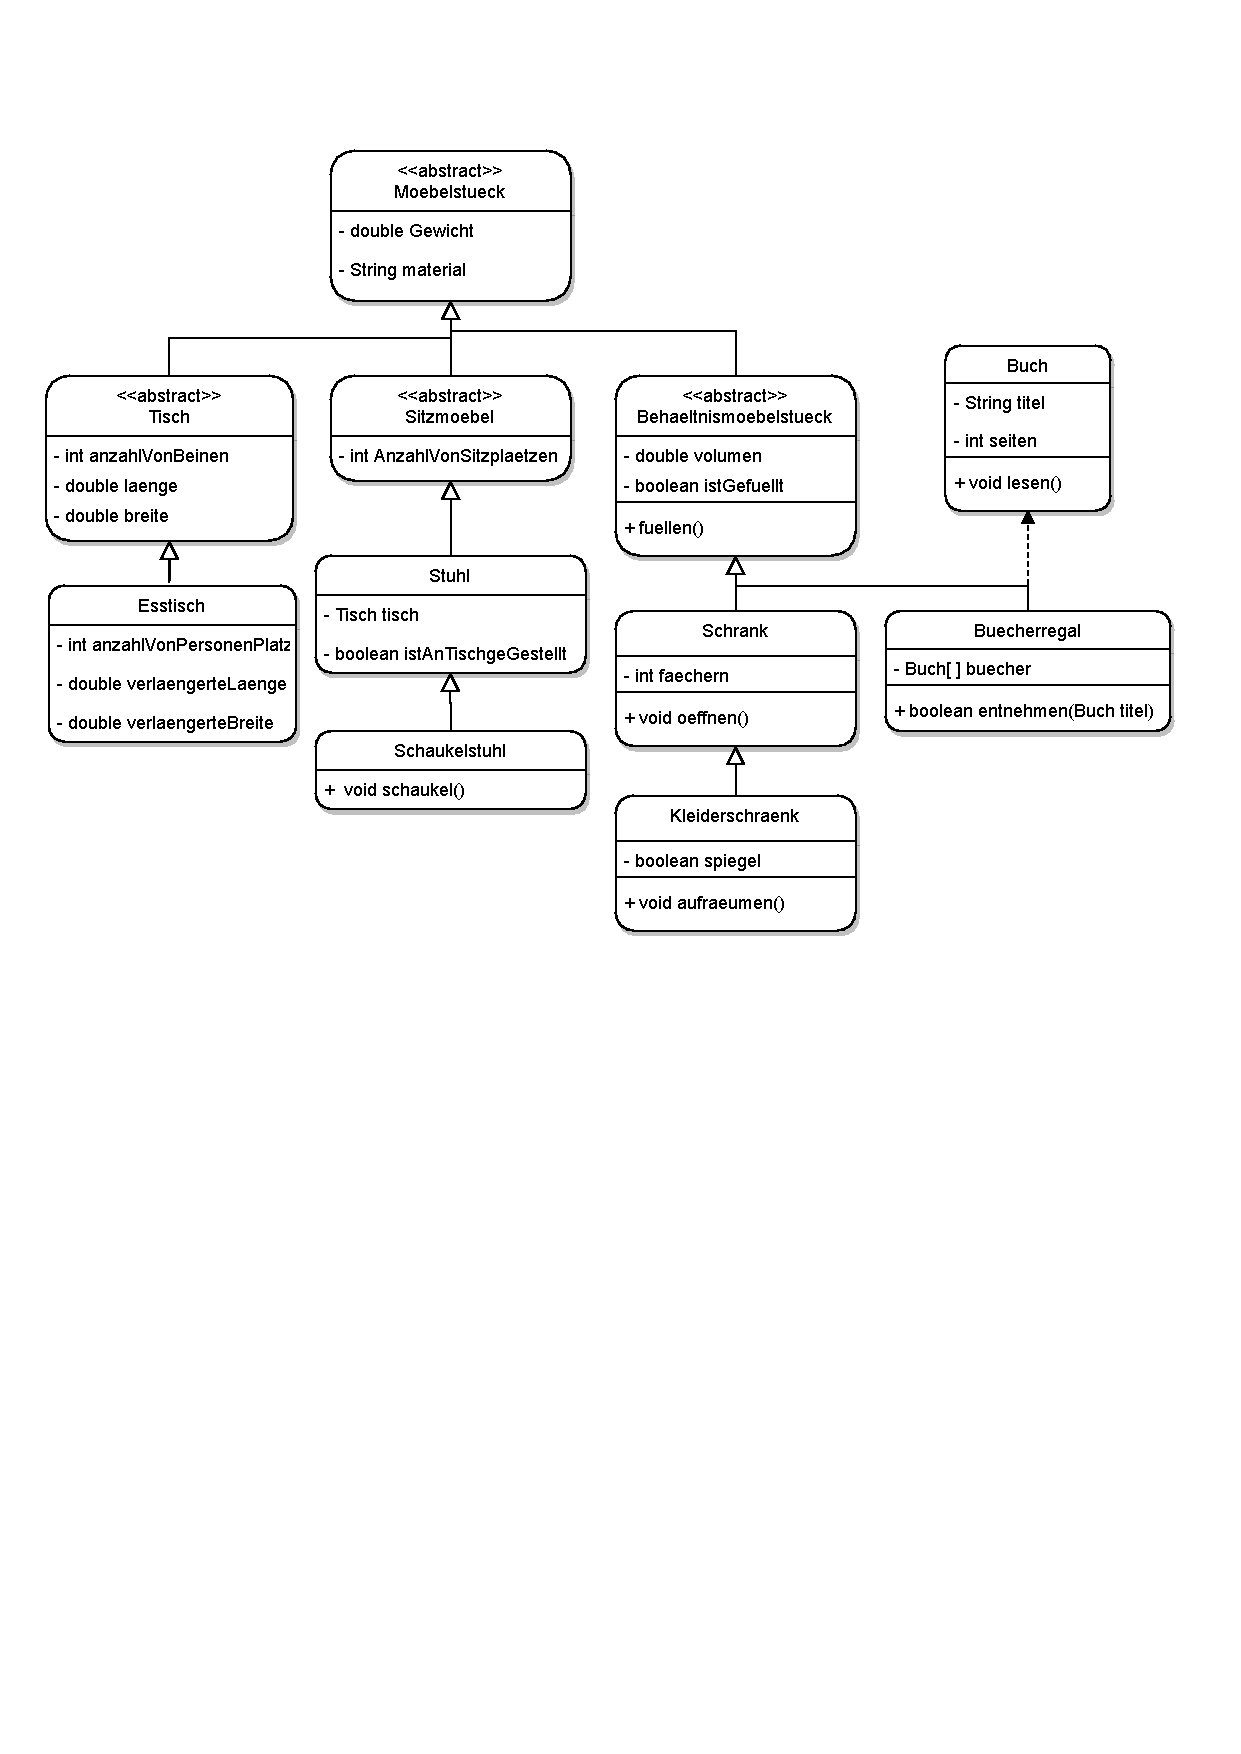
\includegraphics[width=1.25\textwidth]{Moebelstueck.pdf}
		\centering
	\end{figure}

\section*{Aufgabe 5}
\subsection*{a)}
	1)
	\begin{itemize}
		\item A(I) wird explizit aufgerufen mit Parameter 5.
		\item Object() wird durch implizites super() aufgerufen.
		\item A.x wird auf "ubergebenen Wert 5 + 2 (=7) gesetzt(A.x=7). a1.y wird auf übergebenen Wert 7 - 7 (=0) gesetzt(A.y=0).
		\item Es wird 7 und 0 ausgegeben.
	\end{itemize}
	2)
	\begin{itemize}
		\item A() wird explizit aufgerufen.
		\item A(I) wird durch explizites this(...) aufgerufen mit Parameter (int) 7.
		\item Object() wird durch implizites super() aufgerufen.
		\item A.x wird auf "ubergebenen Wert 7 + 2(=9) gesetzt(A.x=9). a2.y wird auf "ubergebenen Wert 7 - 9(=-2) gesetzt(A.y=-2).
		\item A.x wird durch x++ mit 1 addiert.(A.x = 9+1 = 10)
		\item Es wird 10 und -2 ausgegeben.
	\end{itemize}
	3)
	\begin{itemize}
		\item B() wird explizit aufgerufen.
		\item b.x wird durch x++ mit 1 addiert. (B.x = 1.5+1 = 2.5)
		\item A.x : 10
		\item B.x : 2.5
		\item ((A) b).y = 7
		\item B.y: 1
		\item Es wird 10, 2.5, 7 und 1 ausgegeben.
	\end{itemize}
	4)
	\begin{itemize}
		\item B(F) wird explizit aufgerufen, da es kein Konstruktor mit genau passender Signatur gibt und somit der "ubergebene int-Wert mit impliziter Typanpassung in 3.0 float umgewandelt wurde.
		\item A(D) wird durch explizites super(...) aufgerufen mit Parameter 3.0 double, da float-Wert 3.0 mit impliziter Typanpassung in 3.0 double umgewandelt wurde.
		\item Object() wird durch implizites super() aufgerufen.  
		\item A.y wird auf "ubergebenen Wert 7 + 7.0 (=14 int) gesetzt(A.y = 14).
		\item A.y wird durch explizites super.y++ auf 14 + 1(=15 int) gesetzt.
		\item A.y : 15 ; B.y = 1;
		\item Es wird 15 und 1 ausgegeben.
	\end{itemize}


\subsection*{b)}

	1)\\
	\textbf{Parameter}: int, A.		\textbf{a1}: A.  Somit wird die genau passende Methode A.f(IA) aufgerufen.\\
	2)\\
	\textbf{Parameter}: long, A.		\textbf{a1}: A.  Somit wird die genau passende Methode A.f(LA) aufgerufen.\\
	3)\\
	\textbf{Parameter}: int, B.		\textbf{b}: B.  Somit wird die genau passende Methode B.f(IF) aufgerufen.\\
	4)\\
	\textbf{Parameter}: double, A.		\textbf{b}: B. Es gibt keine genau passende Methode in B, aber in A schon. Da B von A erbt, wird A.f(DA) aufgerufen.\\
	5)\\
	\textbf{Parameter}: int, A.		\textbf{ab}: A. Somit wird die genau passende Methode A.f(IA) aufgerufen.\\
	6)\\
	\textbf{Parameter}: int, B.		\textbf{ab}: A. Die Methode A.f(IA) wird aufgerufen, weil B mit impliziter Typanpassung in A umgewandelt wurde.









\rule{\textwidth}{0.2mm}



\section*{Aufgabe 8}

	\begin{lstlisting}[mathescape=true, language=java]

	\end{lstlisting}

\end{document}

